\documentclass[a4paper,12pt]{article}

\usepackage{iftex}
\usepackage[french]{babel}
\usepackage{graphicx}
\usepackage{float}
\usepackage{geometry}
\usepackage{array}

\ifPDFTeX
    \usepackage[utf8]{inputenc}
    \usepackage[T1]{fontenc}
\else
    \usepackage{fontspec}
    \setmainfont{Calibri}
\fi

\geometry{margin=2.5cm}
\setcounter{secnumdepth}{1}
\setcounter{tocdepth}{1}

\begin{document}

\begin{titlepage}
    \thispagestyle{empty}

    \noindent
    \begin{minipage}[t]{0.35\textwidth}
        \vspace{0pt}
        
\includegraphics[width=0.9\textwidth]{img/iut_logo}
    \end{minipage}
    \hfill
    \begin{minipage}[t]{0.55\textwidth}
        \vspace{0pt}
        \begin{flushright}
            \textbf{Universite Paris Est Creteil} \\
            \textbf{IUT Senart Fontainebleau}
        \end{flushright}
    \end{minipage}

    \vspace{2cm}

    \begin{center}
        {\LARGE \textbf{SAE 4.1}}\\[0.5cm]
        {\Huge \textbf{Chuzzle}}\\[0.8cm]
        {\Large Rapport}\\[1.5cm]

        
\includegraphics[width=0.3\textwidth]{img/logo}\\[1.5cm]

        {\large
        Algassimou Pellel DIALLO \\[0.5cm]
        Ayoub ANHDIRE \\[0.5cm]
        Youness BOULALAM
        }
    \end{center}

    \vfill

    \begin{center}
        {\large Date : \today}
    \end{center}
\end{titlepage}

\tableofcontents
\newpage

\section*{Introduction}

Dans le cadre de la SAE 4.1, nous avons conçu et développé une application Android inspirée du jeu de réflexion \textbf{Chuzzle}. Ce projet avait pour objectif de mettre en pratique nos compétences en programmation orientée objet, en conception logicielle et en développement mobile.
Le jeu repose sur une grille de taille 6x6 composée d’éléments colorés. Le joueur peut effectuer des glissements de lignes ou de colonnes afin de former des séries d’au moins trois éléments identiques. Lorsqu’une série est créée, elle est supprimée, les éléments situés au-dessus tombent sous l’effet de la gravité, puis de nouveaux éléments apparaissent. Ce mécanisme peut engendrer des réactions en chaîne, appelées cascades, qui enrichissent la dynamique du jeu.
L’objectif principal est d’obtenir le score le plus élevé possible avant qu’aucun coup ne soit réalisable. Le jeu intègre également plusieurs fonctionnalités supplémentaires telles que la gestion d’une graine pour rejouer une partie identique, un mode difficile augmentant la complexité du gameplay, ainsi qu’un système de sauvegarde permettant de reprendre une partie en cours.
Sur le plan technique, le projet a été structuré selon une architecture MVC Modèle,Vue,Contrôleur afin de séparer clairement la logique métier, l’interface utilisateur et la gestion des interactions. Cette organisation nous a permis de développer une application plus modulaire, maintenable et évolutive.
Ce rapport présente les fonctionnalités développées, la structure du programme ainsi que les choix techniques réalisés au cours du projet.

\section{Repartition des taches}
Le tableau suivant resume la repartition principale du travail entre les membres de l'equipe.

\begin{table}[H]
    \centering
    \begin{tabular}{|>{\raggedright\arraybackslash}p{3cm}|>{\raggedright\arraybackslash}p{11cm}|}
        \hline
        \textbf{Membre} & \textbf{Travail realise} \\
        \hline
        Diallo & Generation sans serie initiale, glissement des colonnes, detection des series, gravite, remplissage, fin de partie, blocage apres fin, mode difficile, sauvegarde et restauration, accessibilite visuelle. \\
        \hline
        Ayoub & Glissement des lignes, validation des coups, suppression des series, resolution complete, bonus de cascade, saisie de la graine et gestion du retour. \\
        \hline
        Youness & Structure de la grille, types d'elements, generateur aleatoire, calcul du score, affichage du score, blocage des lignes et colonnes, affichage de la seed. \\
        \hline
    \end{tabular}
    \caption{Repartition principale des taches}
\end{table}


\newpage



\section{Fonctionnalites}

\subsection{Acces au jeu}

Le menu principal permet de lancer une partie normale, une partie destinee par
graine, d'acceder aux parametres et de quitter l'application.

\begin{figure}[H]
    \centering
    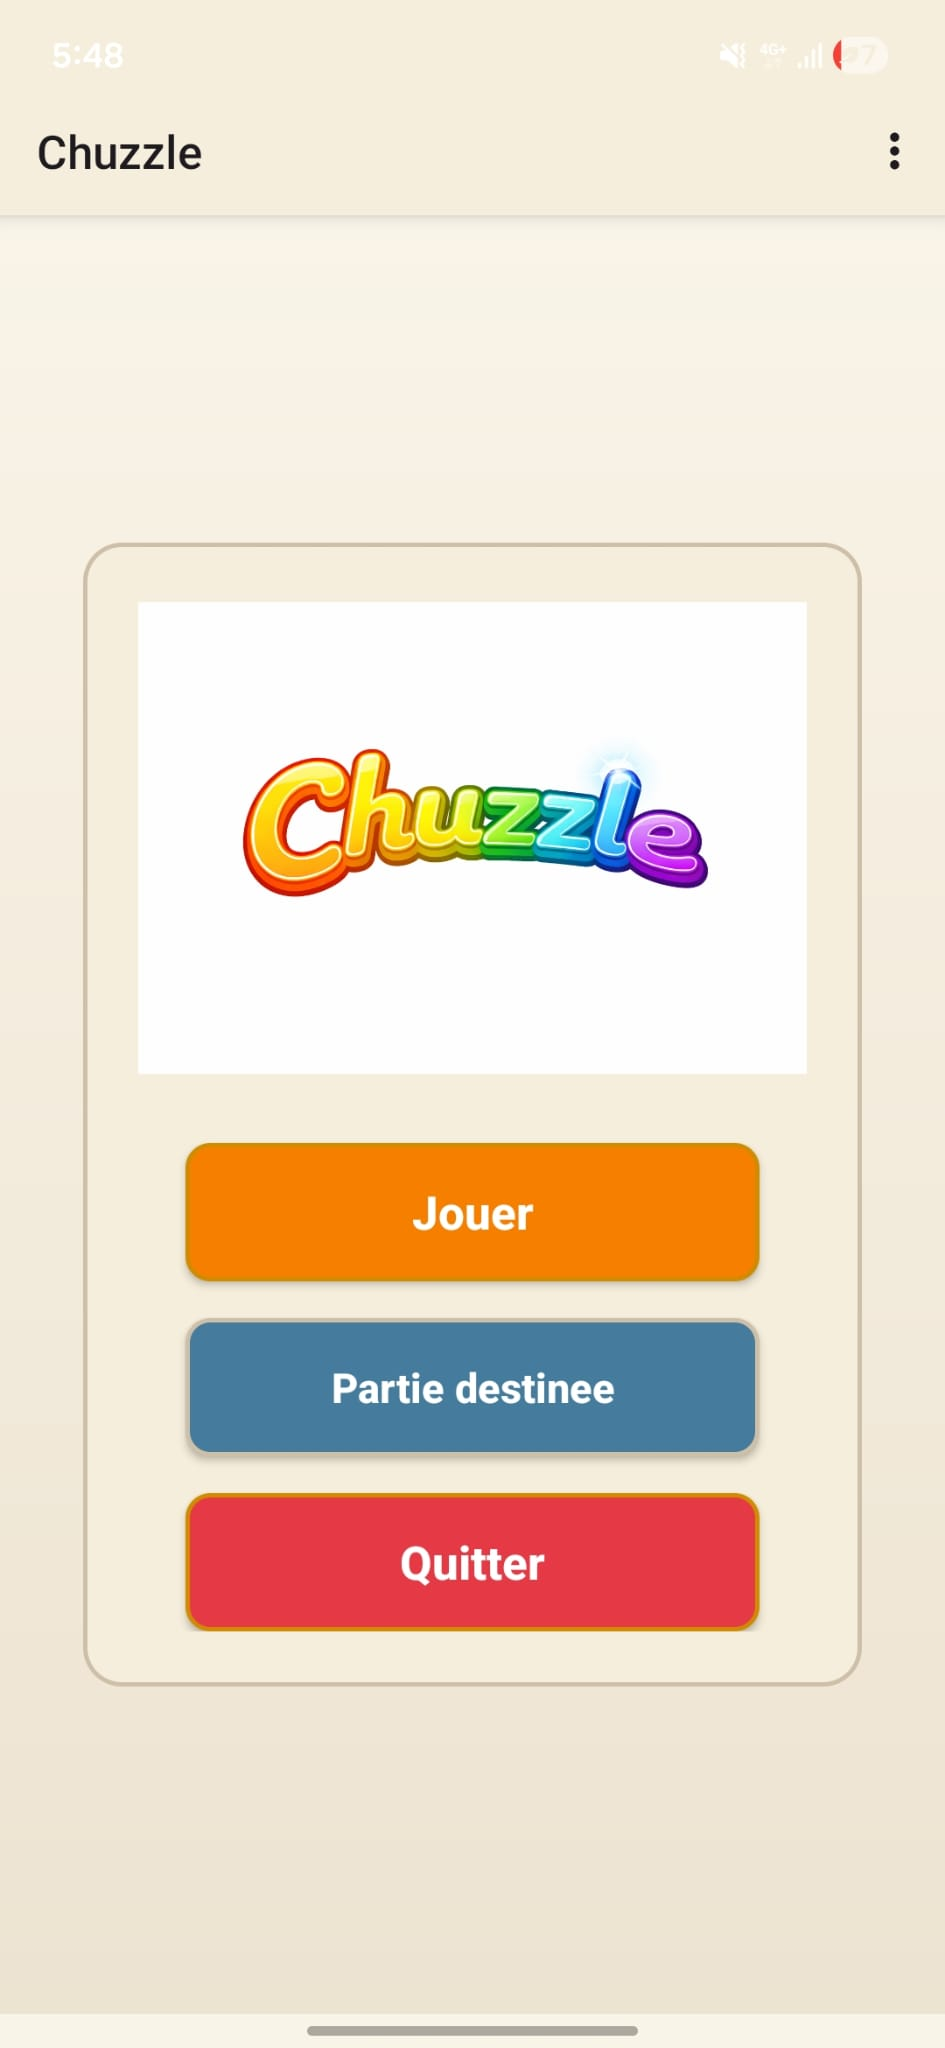
\includegraphics[width=0.55\textwidth]{img/menu.jpeg}
    \caption{Activite de jeu}
\end{figure}


\subsection{Graine}

La graine permet de generer une partie reproductible. En entrant la meme
valeur, le joueur retrouve la meme configuration de depart. Cette
fonctionnalite est utile pour rejouer une situation precise ou pour verifier
le comportement du jeu sur un plateau connu.

\begin{figure}[H]
    \centering
    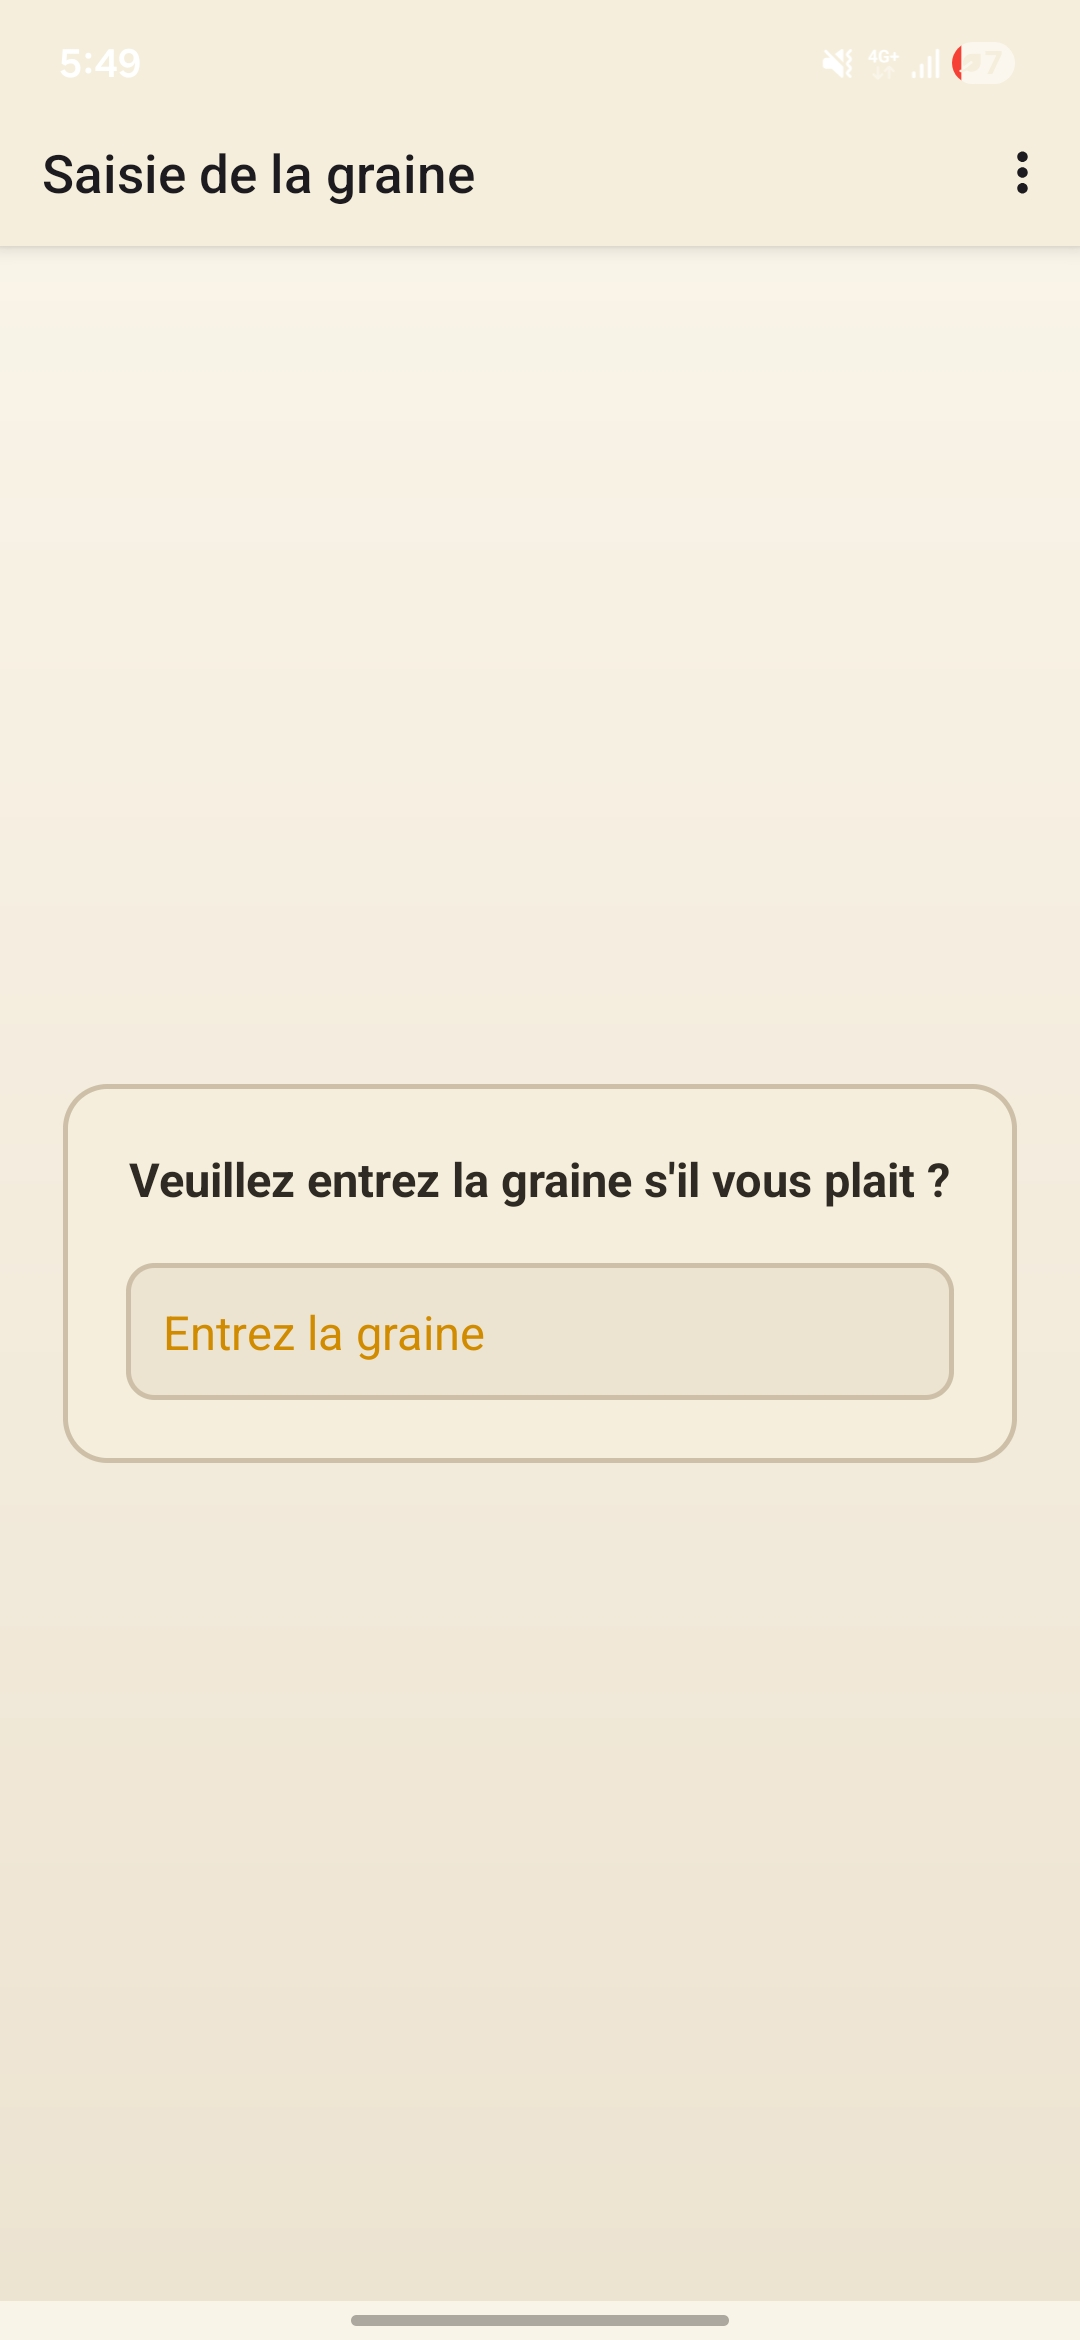
\includegraphics[width=0.45\textwidth]{img/graine.jpeg}
    \caption{Saisie d'une graine}
\end{figure}


\subsection{Deroulement d'une partie}

L'activite de jeu affiche la grille, le score, le nombre de coups et la seed.
Le joueur peut glisser une ligne ou une colonne. Un coup est valide seulement
s'il cree une serie.

\begin{figure}[H]
    \centering
    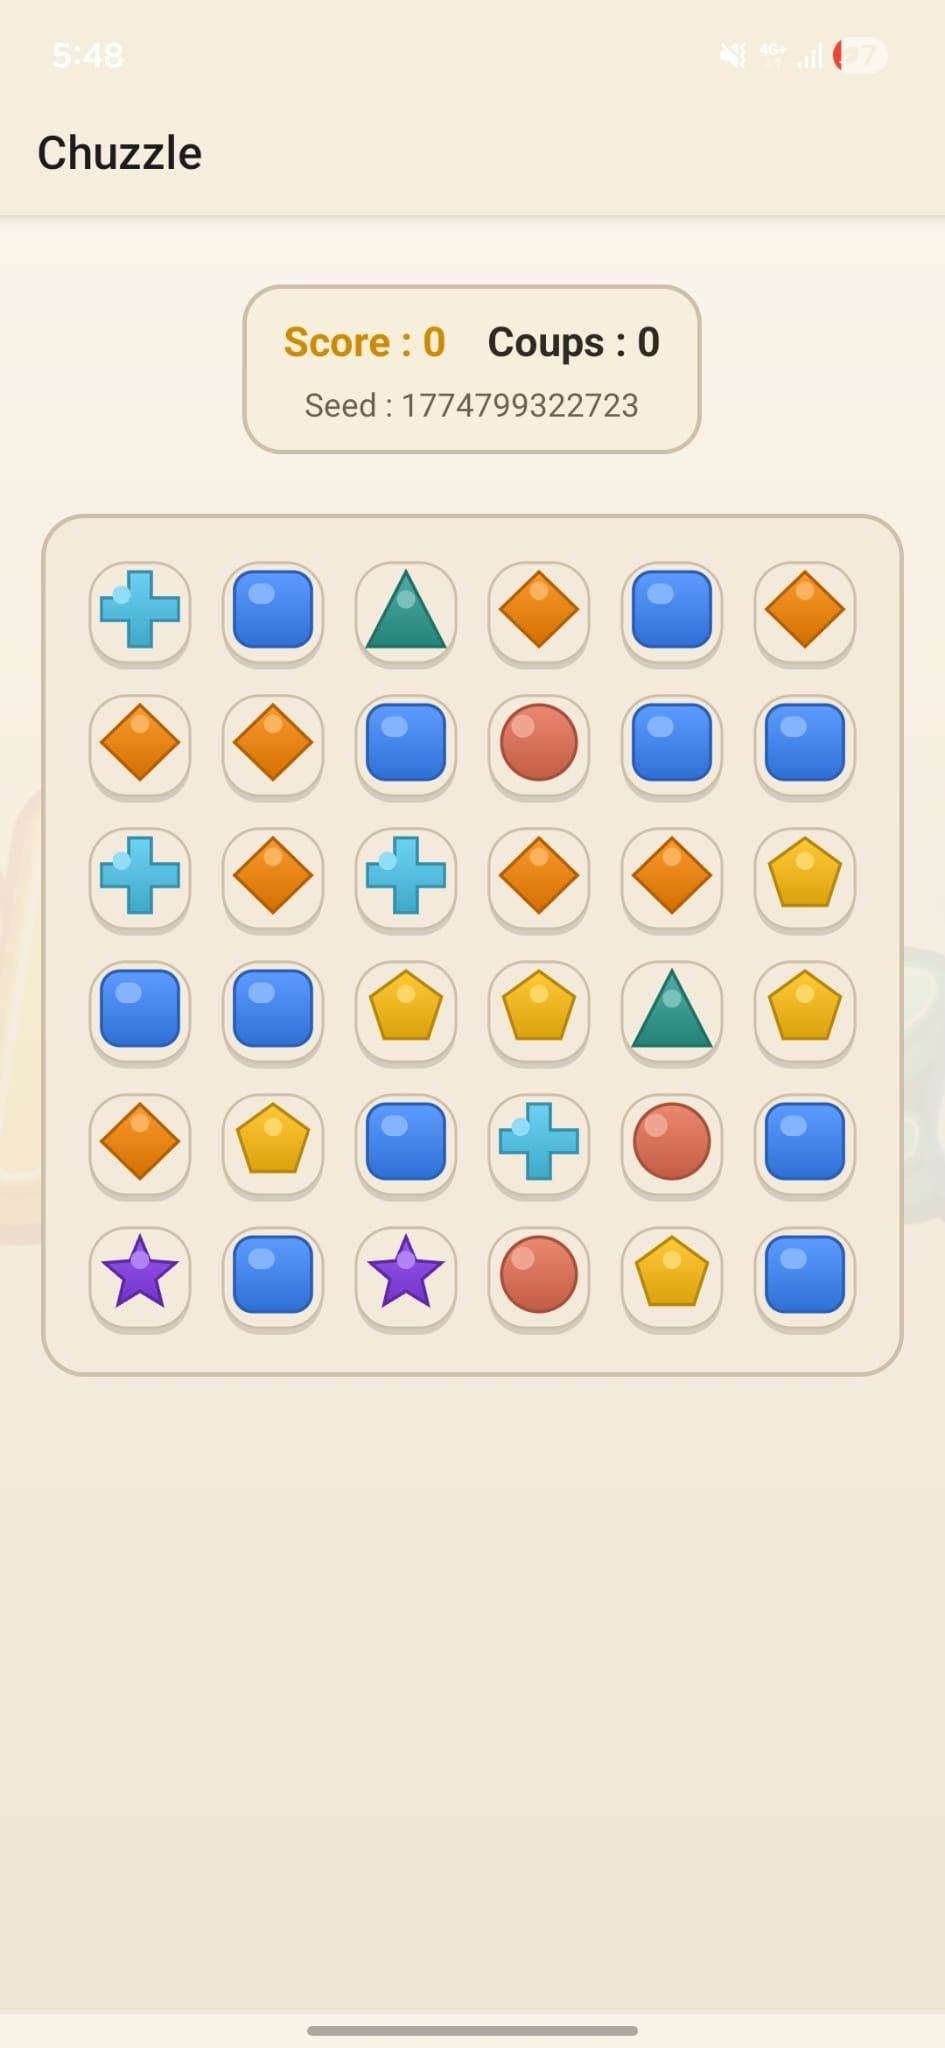
\includegraphics[width=0.55\textwidth]{img/jeu.jpeg}
    \caption{Activite de jeu}
\end{figure}


\subsection{Fin de partie et sauvegarde}

La partie se termine lorsqu'aucun coup n'est possible. La sauvegarde, elle,
intervient lorsque l'application passe en arriere-plan, ce qui permet ensuite
de reprendre la partie plus tard.

\begin{figure}[H]
    \centering
    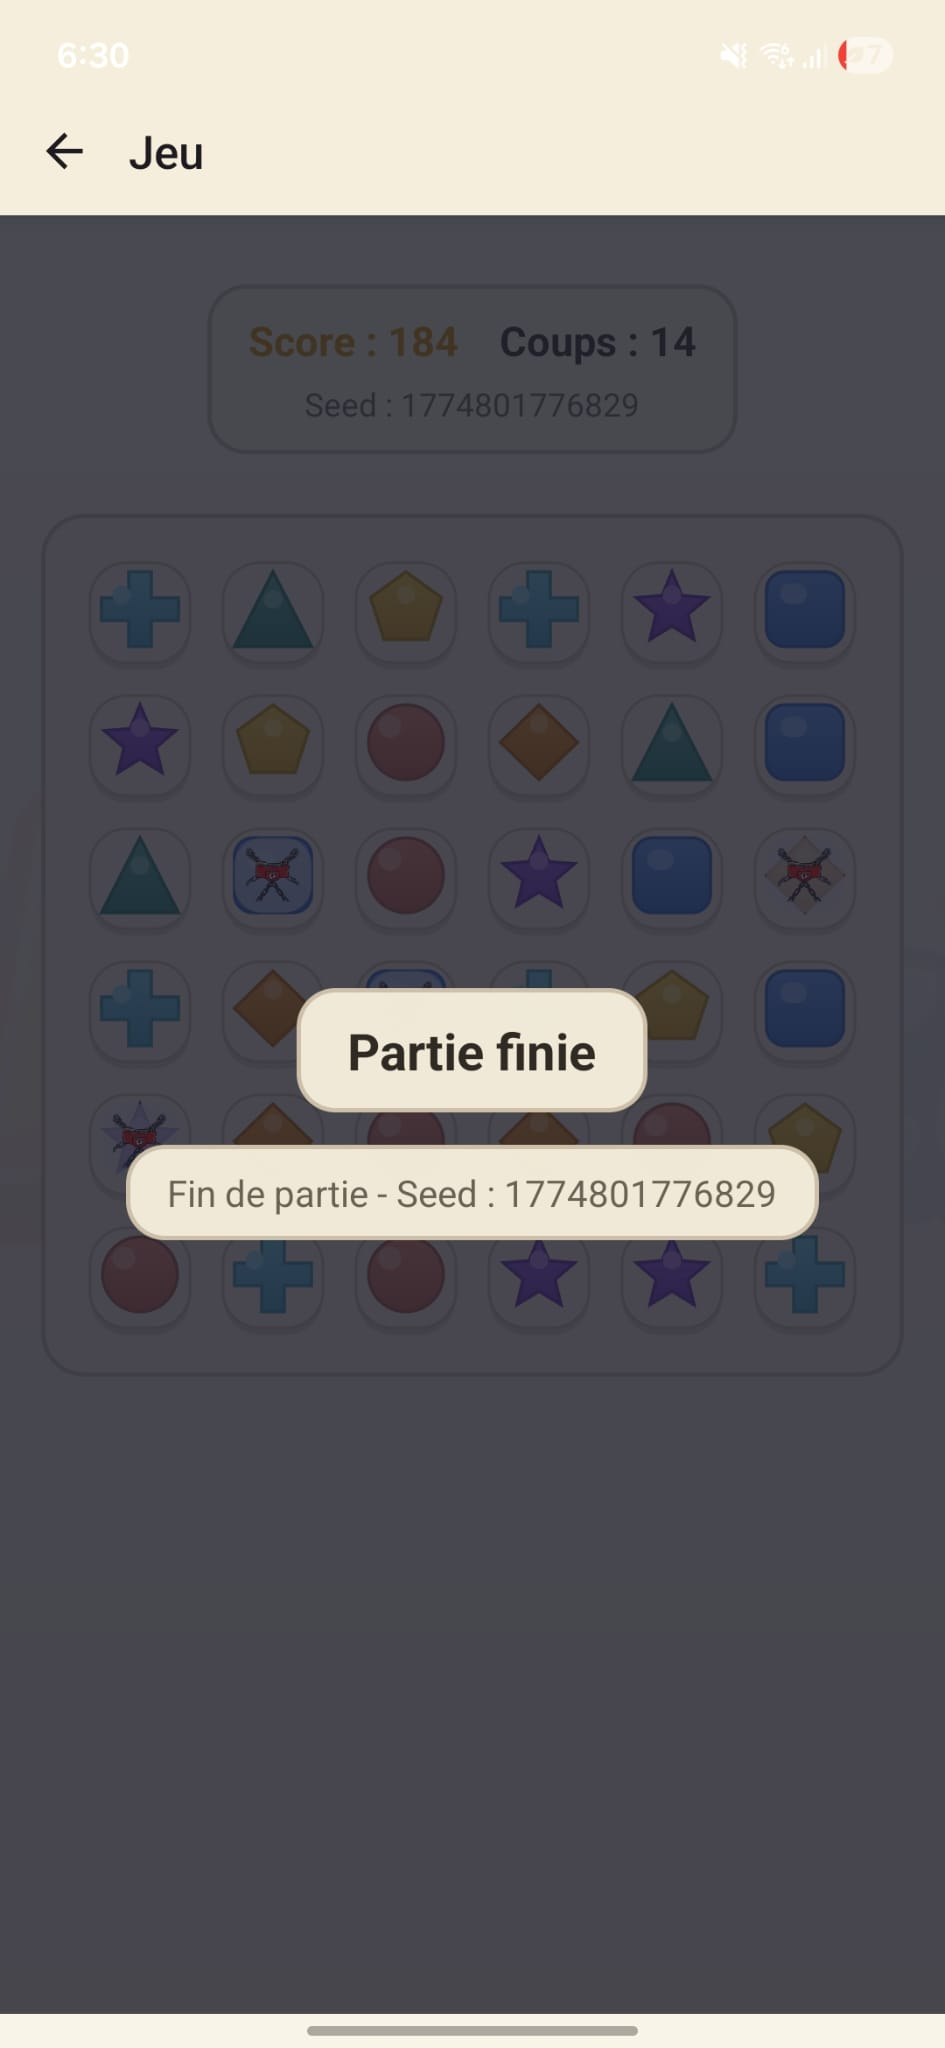
\includegraphics[width=0.55\textwidth]{img/fin.jpeg}
    \caption{Activite de jeu}
\end{figure}



\subsection{Mode difficile}

Le mode difficile est gere par les preferences Android. Il ajoute des verrous
et une case mystere pour rendre la partie plus contraignante. Cette case cache
temporairement son apparence. Si le joueur la place dans une serie avec des
elements identiques, elle disparait comme les autres cases de la serie.

\begin{figure}[H]
    \centering
    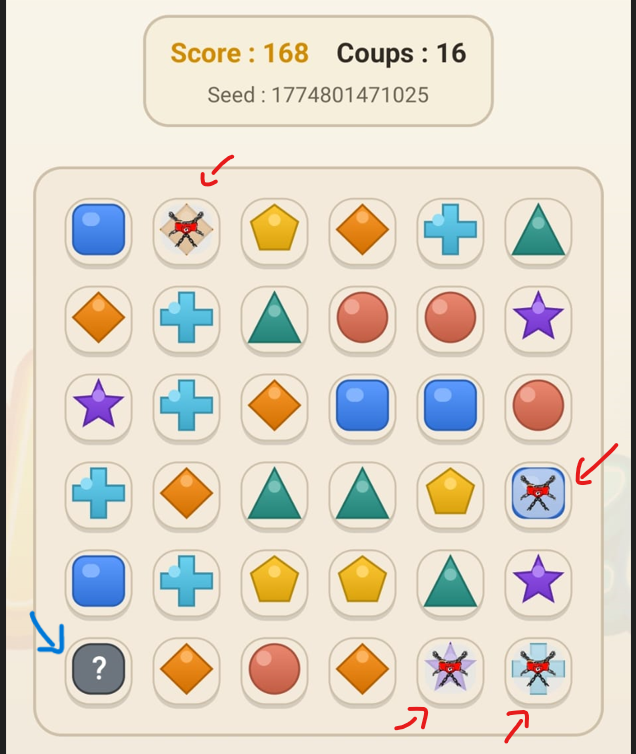
\includegraphics[width=0.55\textwidth]{img/verrou.png}
    \caption{Activite de jeu}
\end{figure}


\section{Structure du programme}

La structure du programme est organisee autour des activites principales de
l'application. Chaque activite correspond a un ecran et s'appuie sur des
classes de controle ou d'ecoute pour traiter les actions de l'utilisateur. Le
fonctionnement general est le suivant : l'activite affiche l'ecran,
l'ecouteur recupere l'action du joueur, puis le controleur ou le moteur
applique le traitement correspondant. Cette organisation permet de separer
l'affichage, la reaction aux interactions et la logique metier du jeu.

\paragraph{ActiviteMenu}
Cette activite affiche le menu principal et utilise \textbf{ControleMenu} et
\textbf{EcouteurMenu}. Son role est de proposer les points d'entree du jeu :
lancement d'une partie normale, acces a la partie destinee, ouverture des
parametres et fermeture de l'application. Concretement, lorsqu'un bouton est
presse, \textbf{EcouteurMenu} detecte le clic puis transmet l'action a
\textbf{ControleMenu}, qui ouvre ensuite l'ecran voulu. Le controleur centralise
donc les transitions de navigation du menu. Cette separation evite de placer
toute la logique de changement d'activite directement dans l'ecran lui-meme.
L'activite reste concentree sur l'affichage des boutons, alors que
\textbf{ControleMenu} decide quoi faire quand l'utilisateur choisit de jouer,
de saisir une graine, d'ouvrir les parametres ou de quitter l'application. On
peut par exemple citer les methodes \texttt{demarrerPartieNormale()},
\texttt{demarrerPartieDestinee()}, \texttt{ouvrirParametres()} et
\texttt{quitterJeu()}.

\begin{figure}[H]
    \centering
    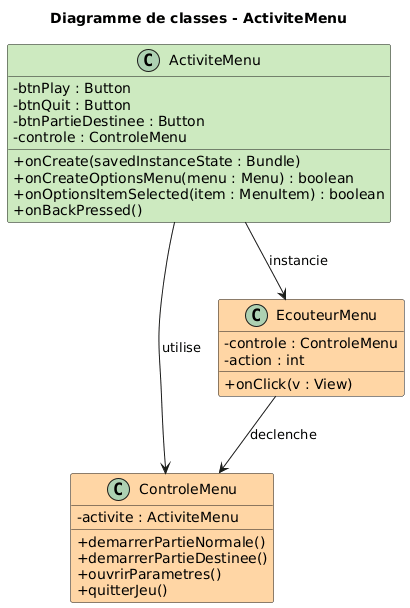
\includegraphics[width=0.55\textwidth]{img/AM}
    \caption{Diagramme de classes de l'activite menu}
\end{figure}

\paragraph{ActiviteGraine}
Cette activite permet de saisir une graine et utilise
\textbf{EcouteurGraine}. Elle sert a recuperer une valeur numerique entree par
l'utilisateur, puis a transmettre cette valeur a l'activite de jeu pour
rejouer une partie reproductible. En pratique, lorsque l'utilisateur valide la
saisie, \textbf{EcouteurGraine} lit le contenu du champ texte, convertit cette
valeur en nombre puis lance la partie avec cette graine. Cette activite a donc
un role simple mais important : elle fait le lien entre la saisie utilisateur
et la creation d'une partie precise. Le passage par une classe d'ecoute permet
de traiter la validation du champ de texte sans surcharger l'activite avec du
code de saisie. Une fois la graine recuperee, l'activite ouvre l'ecran de jeu
en envoyant cette valeur dans l'intent de lancement. La methode
\texttt{demarrerPartieDestinee(long seed)} illustre directement ce passage de
la valeur saisie vers l'ecran de jeu.

\begin{figure}[H]
    \centering
    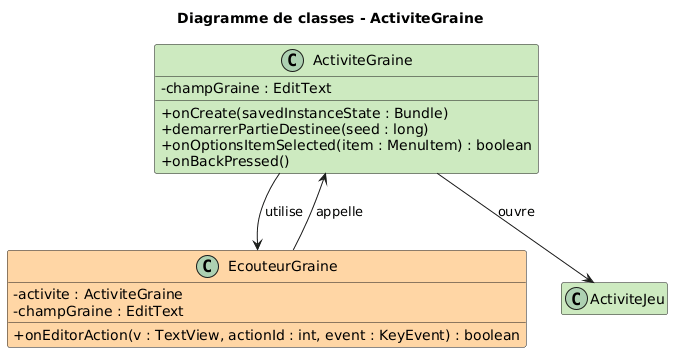
\includegraphics[width=0.55\textwidth]{img/AG}
    \caption{Diagramme de classes de l'activite graine}
\end{figure}

\paragraph{ActiviteJeu}
Cette activite affiche la grille et s'appuie sur \textbf{ControleJeu},
\textbf{EcouteurCase}, \textbf{VueCase} et \textbf{AfficheurNormal}. C'est
l'activite centrale du projet : elle met a jour la grille, le score, la seed,
la fin de partie et transmet les gestes tactiles vers le moteur du jeu par
l'intermediaire du controleur. Concretement, chaque case visible est une
\textbf{VueCase}. Quand le joueur glisse sur une case, \textbf{EcouteurCase}
determine le sens du geste et appelle \textbf{ControleJeu}. Le controleur
transforme ensuite ce geste en deplacement de ligne ou de colonne, puis le
\textbf{MoteurJeu} applique les regles du jeu. Enfin, l'activite relit l'etat
de la grille et rafraichit l'affichage. Cette activite assure aussi plusieurs
taches complementaires : elle lit la seed transmise au lancement, recupere
l'etat du mode difficile depuis les preferences, tente une restauration si une
partie sauvegardee existe, puis construit visuellement la grille en creant une
\textbf{VueCase} pour chaque position. Chaque vue est ensuite associee a un
\textbf{EcouteurCase} afin de capter les glissements tactiles. Lorsqu'un coup
est termine, \textbf{ActiviteJeu} met a jour les textes du score, du nombre de
coups et de la seed, puis verifie si la partie est finie. Si c'est le cas, elle
affiche l'overlay de fin de partie. Cette activite joue donc le role de point
de coordination entre l'interface, les gestes du joueur et le moteur metier.
Les methodes \texttt{initialiserPartie()}, \texttt{initialiserGrille()},
\texttt{actualiserJeu()}, \texttt{afficherCase(...)} et
\texttt{verifierFinPartie()} montrent bien ces differentes responsabilites.
Du cote du controleur et du moteur, les methodes
\texttt{jouerGlissement(...)} et \texttt{jouerCoup(...)} sont au coeur du
traitement d'un mouvement.

\begin{figure}[H]
    \centering
    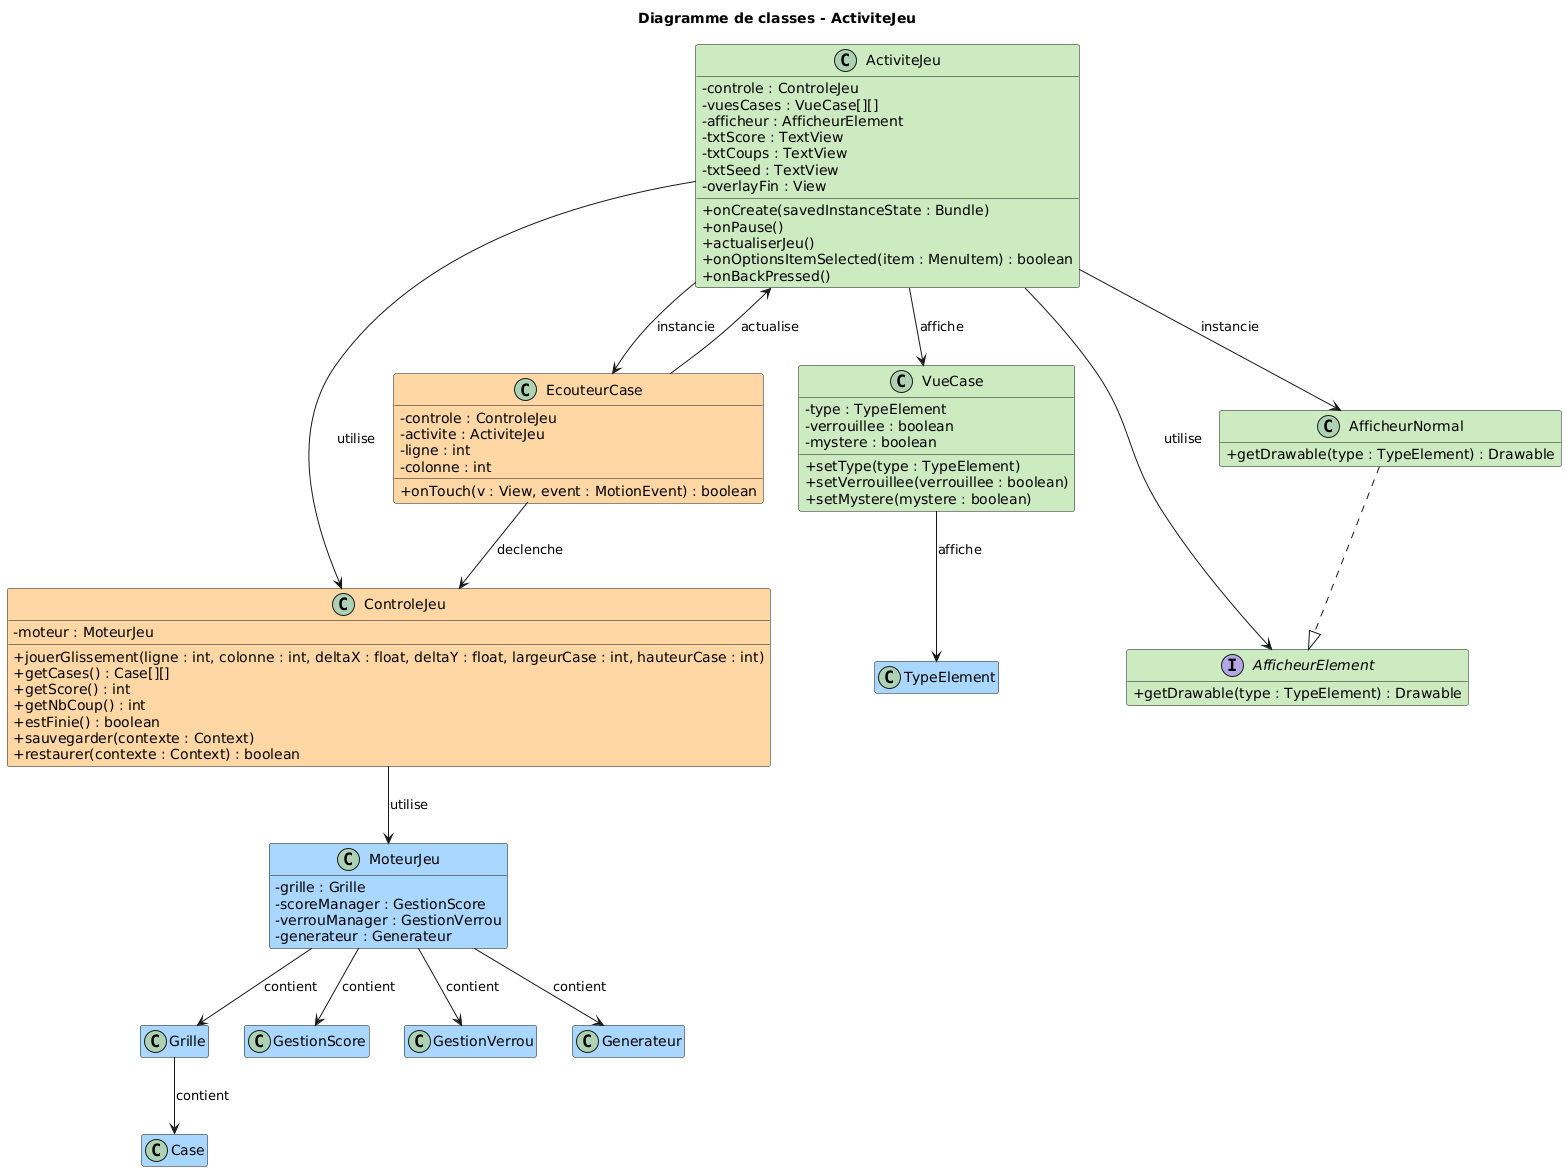
\includegraphics[width=0.55\textwidth]{img/AJ}
    \caption{Diagramme de classes de l'activite jeu}
\end{figure}

\paragraph{ActiviteOptions}
Cette activite gere les preferences Android et utilise
\textbf{ControleOptions} et \textbf{ObservateurPreferences}. Elle permet
d'activer ou de desactiver le mode difficile et de mettre a jour l'affichage
des preferences en fonction de l'etat courant de cette option. En pratique,
l'activite charge le fichier XML de preferences, affiche l'interrupteur du mode
difficile, puis \textbf{ControleOptions} lit la valeur actuelle. Quand la
preference change, \textbf{ObservateurPreferences} met a jour le resume affiche.
Cette activite sert donc de point d'acces aux reglages persistants du jeu. Le
choix de passer par les preferences Android permet de conserver l'etat du mode
difficile entre deux lancements de l'application. Le controleur isole la lecture
de cette valeur, tandis que l'observateur garantit une mise a jour immediate de
l'interface quand l'utilisateur change l'option. Les methodes
\texttt{actualiserResumeModeDur()} et \texttt{isHardMode()} sont les plus
representatives de ce fonctionnement.

\begin{figure}[H]
    \centering
    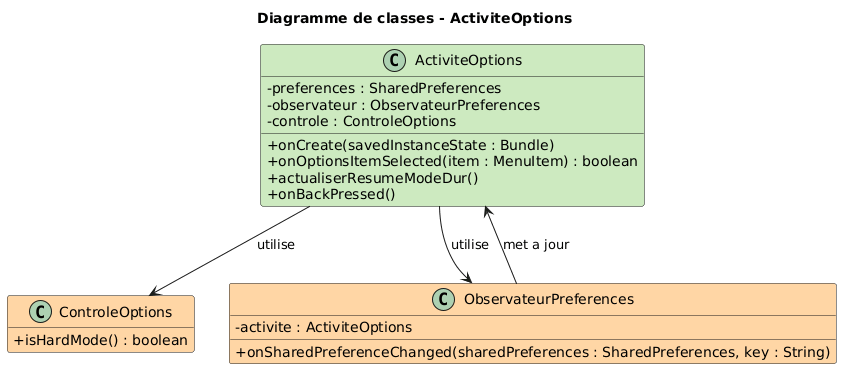
\includegraphics[width=0.55\textwidth]{img/AO}
    \caption{Diagramme de classes de l'activite options}
\end{figure}

\section{Algorithme de fin de partie}

La fin de partie est detectee en verifiant s'il reste au moins un coup valide
sur la grille. L'algorithme utilise pour cette verification ne se contente pas
de regarder l'etat courant du plateau : il simule les deplacements possibles
afin de savoir si l'un d'eux pourrait creer une serie.
Concretement, la methode \texttt{Grille.existeCoupPossible()} parcourt chaque
ligne puis chaque colonne de la grille. Pour chaque ligne ou colonne
glissable, elle teste plusieurs decalages possibles sur une copie du plateau.
Apres chaque simulation, elle appelle la detection des series pour verifier si
une combinaison de trois elements identiques ou plus apparait. Si une seule
simulation produit une serie, alors la methode conclut qu'un coup reste
possible et la partie continue.
Dans le cas contraire, si toutes les lignes et toutes les colonnes ont ete
testees sans qu'aucun glissement ne cree de serie, la grille est consideree
comme bloquee. Le moteur met alors l'etat de fin de partie a \texttt{true}.
Cette verification est relancee apres l'initialisation de la grille et apres
chaque coup valide, ce qui garantit que la partie se termine exactement au
moment ou plus aucun coup ne peut etre joue.

\section{Conclusion}

\subsection{Algassimou Pellel DIALLO}
Ce projet m'a permis de progresser dans plusieurs aspects du developpement
Android. J'ai notamment travaille sur la logique du jeu, la gestion de la
grille, la fin de partie et la sauvegarde.
Au debut, j'avais du mal avec le systeme de preferences Android, en
particulier leur mise en place et leur utilisation dans le projet. Avec ce
travail, j'ai pu mieux comprendre leur fonctionnement et apprendre a les
maitriser de facon plus correcte.
Cette SAE m'a aussi permis de mieux comprendre l'importance d'une bonne
organisation du code et du travail en equipe. Elle m'a donne plus d'aisance
dans le developpement d'une application Android complete.


\subsection{Ayoub ANHDIRE}
Au cours de ce projet, j'ai surtout travaille sur des parties importantes de la
logique du jeu, comme le glissement des lignes, la validation des coups, la
suppression des series, la resolution complete d'un tour et le bonus de
cascade. J'ai aussi participe a la saisie de la graine et a la gestion du
retour entre les activites.
Ce travail m'a permis de mieux comprendre comment relier les regles d'un jeu a
leur implementation concrete dans le code. J'ai particulierement appris a bien
reflechir au deroulement complet d'un coup, depuis l'action du joueur jusqu'a la
mise a jour finale de la grille et du score.
Cette SAE m'a aussi aide a progresser en developpement Android,
notamment sur la logique de navigation entre les ecrans. Elle m'a montre qu'un
petit detail dans les regles du jeu peut avoir un impact important sur tout le
fonctionnement du programme.

\subsection{Youness BOULALAM}

Ma contribution à ce projet a principalement porté sur la mise en place du générateur
de types aléatoires, le calcul du score de base, l'affichage des informations de jeu
à l'écran ainsi que sur les aspects liés à l'accessibilité visuelle.
La réalisation de l'affichage daltonien a constitué pour moi le défi le plus stimulant
de ce projet. Il ne s'agissait pas uniquement d'un problème technique, mais d'une
réflexion plus large sur la conception d'une interface : différencier les
éléments par la forme autant que par la couleur Suite à vos explications, nous avons constaté que l’utilisation des couleurs seules n’était pas suffisante et qu’il était nécessaire d’ajouter un élément visuel plus distinctif.
Ce projet m'a permis de consolider mes compétences en développement Android,
notamment dans la manipulation du Canvas et la gestion du cycle de vie des activités.
Il m'a également sensibilisé à l'importance d'une architecture bien définie dès le
départ, sans laquelle la coordination entre les membres de l'équipe aurait été
considérablement plus difficile.
À titre d'amélioration, il serait intéressant d'enrichir l'expérience visuelle par
des animations lors de la suppression des séries.



\end{document}
